\documentclass{beamer}

\usetheme{Madrid}

\usepackage{graphicx}
\usepackage{booktabs}
\usepackage[italian]{babel}

\title{Intrusion Detection sul dataset UNSW-NB15}
\subtitle{Classificazione Binaria e Multiclasse del Traffico di Rete}
\author{Simone Montagnini}
\institute{Università di Bologna}
\date{Settembre 2026}

\begin{document}

\frame{\titlepage}

\begin{frame}{Indice}
  \tableofcontents
\end{frame}

\section{Introduzione}

\begin{frame}{Obiettivi del Progetto}
  Questo progetto affronta il rilevamento delle intrusioni nel traffico di rete attraverso due task di classificazione:
  \begin{itemize}
    \item \textbf{Classificazione binaria}: distinzione tra traffico normale e malevolo
      (\texttt{label})
    \item \textbf{Classificazione multiclasse}: identificazione della minaccia specifica tra 9 possibili tipologie (\texttt{attack\_cat})
  \end{itemize}
  \vspace{0.5cm}
  \begin{block}{Sorgente}
  Competizione Kaggle: \href{https://www.kaggle.com/competitions/advanced-ai-for-cybersecurity-intrusion-detection-with-unsw-nb-15/overview}{\textit{Advanced AI for Cybersecurity — Intrusion Detection with UNSW-NB15}}
  \end{block}
\end{frame}

\begin{frame}{Il Dataset — UNSW-NB15}
  \begin{itemize}
    \item Dataset di traffico di rete realistico contenente attività sia normali che malevole
    \item \textbf{175.341} record di training, \textbf{42} feature iniziali
      (categoriche e numeriche)
    \item Due colonne target:
      \begin{itemize}
        \item \texttt{label}: 0 = normale, 1 = attacco
        \item \texttt{attack\_cat}: Normal, Generic, Exploits, Fuzzers, DoS,
          Reconnaissance, Analysis, Backdoor, Shellcode, Worms
      \end{itemize}
  \end{itemize}
\end{frame}

\section{Analisi Esplorativa dei Dati}

\begin{frame}{Distribuzione del Target}
  \begin{columns}
    \column{0.5\textwidth}
    \textbf{Binaria (\texttt{label})}
    \begin{itemize}
      \item Attacco: 68.1\%
      \item Normale: 31.9\%
    \end{itemize}

    \column{0.5\textwidth}
    \textbf{Multiclasse (\texttt{attack\_cat})}
    \begin{itemize}
      \footnotesize
      \item Normal: 56.000
      \item Generic: 40.000
      \item Exploits: 33.393
      \item Fuzzers: 18.184
      \item DoS: 12.264
      \item Reconnaissance: 10.491
      \item Analysis: 2.000
      \item Backdoor: 1.746
      \item Shellcode: 1.133
      \item \textbf{Worms: 130}
    \end{itemize}
  \end{columns}
  \vspace{0.3cm}
  \begin{alertblock}{Sbilanciamento}
    Il target binario è relativamente bilanciato, ma \texttt{attack\_cat} presenta forti sbilanciamenti: la classe Worms è \textbf{430 volte meno numerosa} rispetto a Normal; da qui la necessità di strategie di \textbf{class-weighting} nel modello multiclasse.
  \end{alertblock}
\end{frame}

\begin{frame}{Qualità dei Dati}
  \begin{itemize}
    \item \textbf{Righe duplicate}: 78.519 su 175.341 (\textbf{44,8\%})
      \begin{itemize}
        \item Rimosse prima dello split, così da evitare data leakage tra train e test
      \end{itemize}
    \vspace{0.3cm}
    \item \textbf{Feature categoriche}:
      \begin{itemize}
        \item \texttt{proto} (Alta cardinalità): 133 valori unici (\texttt{tcp}/\texttt{udp}
          $\approx$ 82\% del traffico)
        \item \texttt{service}: 13 valori, 54\% mancanti/sconosciuti (\texttt{-})
        \item \texttt{state}: 9 valori
      \end{itemize}
  \end{itemize}
\end{frame}

\begin{frame}{Feature Numeriche Asimmetriche}
  Diverse feature del traffico presentano distribuzioni right-skewed:
  \begin{center}
    \begin{tabular}{lr}
      \toprule
      \textbf{Feature} & \textbf{Asimmetria} \\
      \midrule
      trans\_depth & 167.3 \\
      response\_body\_len & 76.3 \\
      sbytes & 45.3 \\
      sloss & 44.8 \\
      dloss & 41.4 \\
      spkts & 40.2 \\
      \bottomrule
    \end{tabular}
  \end{center}
  \vspace{0.3cm}
  \textbf{27 feature} superano il limite ($> 1.0$) e subiranno una trasformazione logaritmica (\texttt{log1p}) in fase di preprocessing.
\end{frame}

\section{Preprocessing}

\begin{frame}{Preparazione \& Trasformazione Dati}
  \begin{enumerate}
    \item \textbf{Rimozione duplicati}: rimosse 78.519 righe duplicate prima dello split
    \item \textbf{Split train/test}: 67/33, stratificato su \texttt{label}
    \item \textbf{Encoding}: \texttt{OneHotEncoder} su \texttt{proto},
      \texttt{service}, \texttt{state} — 185 feature totali
    \item \textbf{Correzione asimmetria}: trasformazione \texttt{log1p} su 27 feature (asimmetria $> 1.0$)
  \end{enumerate}
\end{frame}

\begin{frame}{Prevenzione Data Leakage}
  \begin{alertblock}{Scelta chiave}
    Le operazioni di preprocessing eseguono il \textbf{fit solamente sul training set} e vengono applicate sul test set grazie a \texttt{transform()} così da evitare data leakage.
  \end{alertblock}
  \vspace{0.3cm}
  \begin{itemize}
    \item \textbf{Netta separazione}: Fare il fit degli encoder sull'intero dataset  inietta conoscenza futura nella fase di addestramento
    \item \textbf{Gestione dati mai visti}: Categorie rare (e.g. all'interno dei 133 valori di \texttt{proto}) potrebbero apparire solamente nel test set
    \item \textbf{Tolleranza ai guasti}: \texttt{OneHotEncoder} è configurato con \texttt{handle\_unknown='ignore'} per aggirare nuove categorie senza causare blocchi durante l'esecuzione
  \end{itemize}
\end{frame}

\section{Selezione degli attributi}

\begin{frame}{SelectKBest}
  \begin{itemize}
    \item \textbf{Feature selection supervisionata}: ogni feature viene valutata rispetto al target, mantenendo solamente le migliori $k$ feature
\item \textbf{Funzione di score}: ANOVA F-value (\texttt{f\_classif})
      \begin{itemize}
        \item \texttt{mutual\_info\_classif} è stata esclusa a causa del costo computazionale eccessivo data la dimensione del dataset.
      \end{itemize}
    \item \textbf{Selezione}: $k = 50$ su 185 feature, selezionate separatamente per \texttt{label} e \texttt{attack\_cat}
  \end{itemize}
  \vspace{0.3cm}
  \begin{block}{Preservazione dell'Interpretabilità}
    SelectKBest mantiene gli attributi originali del traffico. In questo modo il modello rimane trasparente, permettendo di ricondurre direttamente le attività malevole a specifici segnali di rete.
  \end{block}
\end{frame}

\begin{frame}{PCA}
  \begin{itemize}
    \item \textbf{Scaling preliminare}: feature standardizzate (\texttt{StandardScaler}), con fit della PCA esclusivamente 
      sul training set
    \item \textbf{Varianza spiegata}: mantenere il 90\% della varianza richiede \textbf{137 componenti} (118 per l'80\%) 
    \item \textbf{Riduzione limitata}: le componenti mantenute rappresentano ancora circa il 74\% delle feature originali
  \end{itemize}
  \vspace{0.3cm}
  \begin{block}{Analisi delle Componenti e Contributo delle Feature}
    Piuttosto che essere dominate dalle numerose colonne \texttt{proto} codificate con one-hot encoding, le componenti principali mostrano un mix di tipologie di dati sottostanti. Per esempio, la PC2 è guidata quasi interamente da feature legate alle tempistiche e ai byte (\texttt{sinpkt}, \texttt{dload}, \texttt{tcprtt})
  \end{block}
\end{frame}

\begin{frame}{Confronto sulla Selezione delle Feature}
    \small
    \begin{tabular}{lcc}
      \toprule
       & \textbf{SelectKBest} & \textbf{PCA} \\
      \midrule
      Dimensionalità & 50 feature & 137 componenti \\
      Interpretabilità & Alta (dominio originale) & Bassa (combinazioni lineari) \\
      Trasformazione & Supervisionata (target-aware) & Non supervisionata \\
      Efficienza di training & Accettabile & Proibitiva \\
      \bottomrule
    \end{tabular}
  \vspace{0.5cm}
  \begin{alertblock}{Scelta di Progettazione}
    PCA è stata esclusa dalla pipeline di classificazione: anche con un numero ridotto di componenti, l'overhead computazionale durante la \texttt{GridSearchCV} è risultato proibitivo. Pertanto, la classificazione procede solamente con SelectKBest.
  \end{alertblock}
\end{frame}

\section{Classificazione}

\begin{frame}{Metodologia di Classificazione}
  \begin{itemize}
    \item \textbf{Algoritmi}: Decision Tree (come baseline) e Random Forest
    \item \textbf{Tuning degli Iperparametri}: \texttt{max\_depth} e \texttt{criterion} per Decision Tree, \texttt{n\_estimators} e \texttt{max\_depth} per Random Forest, \texttt{class\_weight} \texttt{None} vs \texttt{'balanced'} per entrambi
    \item \textbf{Gestione dello Sbilanciamento}: incluso \texttt{class\_weight} (\texttt{None} vs \texttt{'balanced'}) per valutare la strategia migliore sui vettori di minaccia rari
    \item \textbf{Validazione}: 5-fold \texttt{StratifiedKFold} per garantire una rappresentazione proporzionale di tutte le classi durante il training
  \end{itemize}
  \vspace{0.2cm}
  \begin{block}{Metriche di Valutazione}
    L'Accuracy è fuorviante su dataset fortemente sbilanciati. I modelli sono valutati sulla base di \textbf{F1-Score} (classificazione binaria) e \textbf{Macro F1-Score} 
    (classificazione multiclasse) per pesare correttamente le performance sulle classi minoritarie.
  \end{block}
\end{frame}

\begin{frame}{Risultati Classificazione Binaria}
  \begin{columns}
    \column{0.5\textwidth}
    \hspace{1.1cm}\textbf{Performance Modello} \\
    \vspace{0.2cm}
    \small
    \hspace{0.5cm}
    \begin{tabular}{lcc}
      \toprule
      \textbf{Metrica} & \textbf{DT} & \textbf{RF} \\
      \midrule
      Accuracy & 0.916 & 0.920 \\
      Precision & 0.918 & 0.923 \\
      Recall & 0.916 & 0.920 \\
      \textbf{F1-Score} & \textbf{0.916} & \textbf{0.920} \\
      \bottomrule
    \end{tabular}

    \vspace{0.1cm}
    \hspace{0.8cm}{\tiny DT = Decision Tree, RF = Random Forest}
    
    \vspace{0.4cm}
    \begin{itemize}
      \item Random Forest raggiunge un eccellente F1-Score di \textbf{0.920}.
      \item Il modello è \textbf{molto affidabile} nella distinzione delle attività malevole dal traffico normale.
    \end{itemize}

    \column{0.5\textwidth}
    \begin{figure}
      \centering
      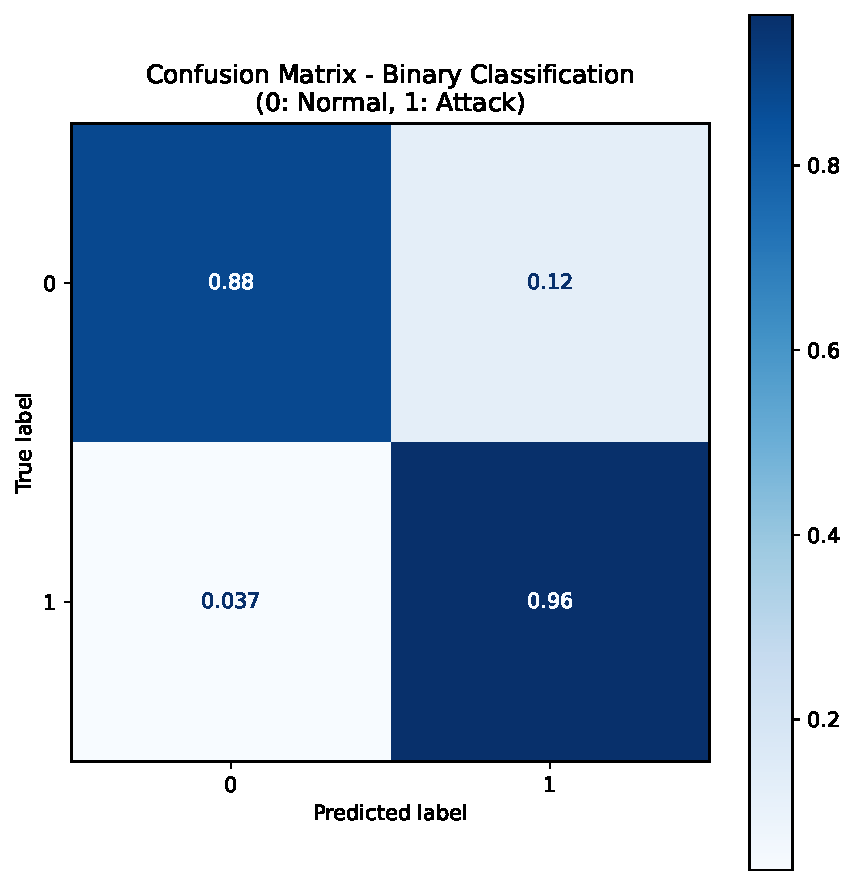
\includegraphics[height=0.65\textheight]{images/cm_binary.pdf}
      \caption{Matrice di Confusione Binaria}
    \end{figure}
  \end{columns}
\end{frame}

\begin{frame}{Risultati Classificazione Multiclasse}
  \begin{columns}
    \column{0.55\textwidth}
    \small
    \textbf{La sfida Multiclasse} \\
    \vspace{0.2cm}
    \begin{itemize}
      \item Il modello migliore ottiene un \textbf{Macro F1-Score} di \textbf{0.57}
      \item Le \textbf{classi più frequenti} (Normal, Generic) vengono predette con alta confidenza
      \item Le \textbf{classi rare} abbassano la media macro a causa della sovrapposizione delle feature e della scarsità di esempi per l'addestramento
    \end{itemize}
    \begin{alertblock}{Impatto del Bilanciamento}
      Grazie a \texttt{class\_weight='balanced'}, il modello riesce a rilevare anche istanze di attacchi molto rari 
      (come Worms), evitando quindi che vengano completamente ignorate.
    \end{alertblock}

    \column{0.45\textwidth}
    \begin{figure}
      \centering
      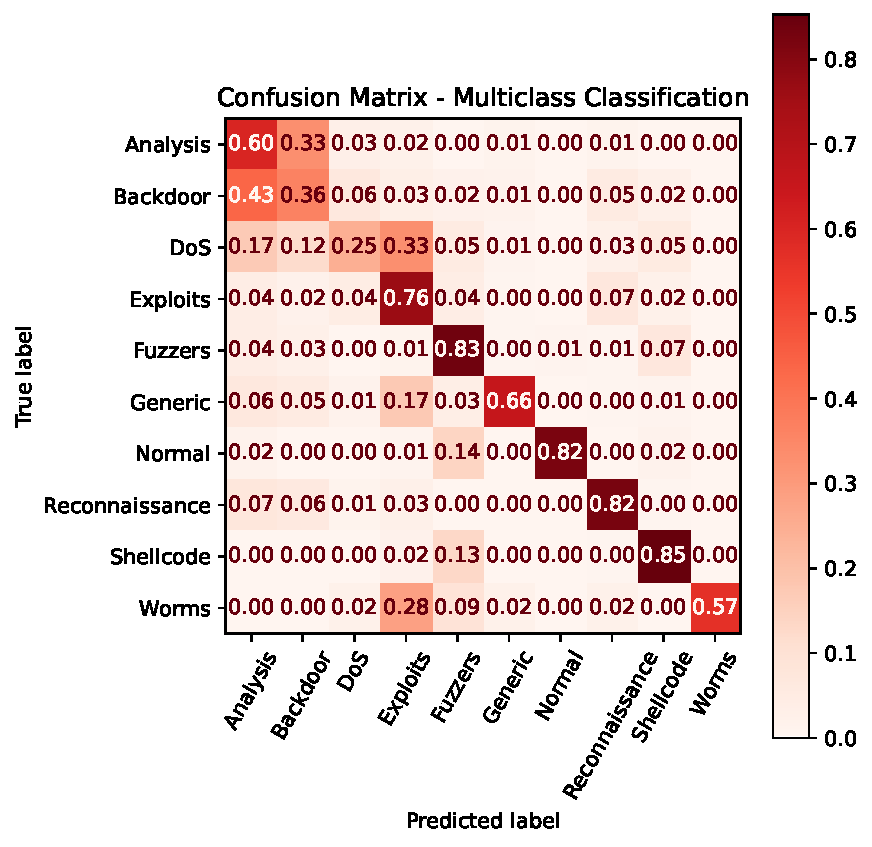
\includegraphics[width=\textwidth]{images/cm_multiclass.pdf}
      \caption{Matrice di Confusione Multiclasse}
    \end{figure}
  \end{columns}
\end{frame}

\begin{frame}{Analisi Feature Importance}
  \begin{itemize}
    \item \textbf{Task binario}: si basa prevalentemente sulle feature temporali del TCP handshake (\texttt{ackdat}, \texttt{synack}, \texttt{tcprtt}): gli handshake anomali rappresentano un forte indicatore di traffico malevolo
    \item \textbf{Task multiclasse}: si affida a feature volumetriche legate al trasferimento di byte (\texttt{sbytes}, \texttt{smean}, \texttt{dbytes}) per distinguere il \textit{tipo} di attacco 
  \end{itemize}

  \vspace{0.3cm}
  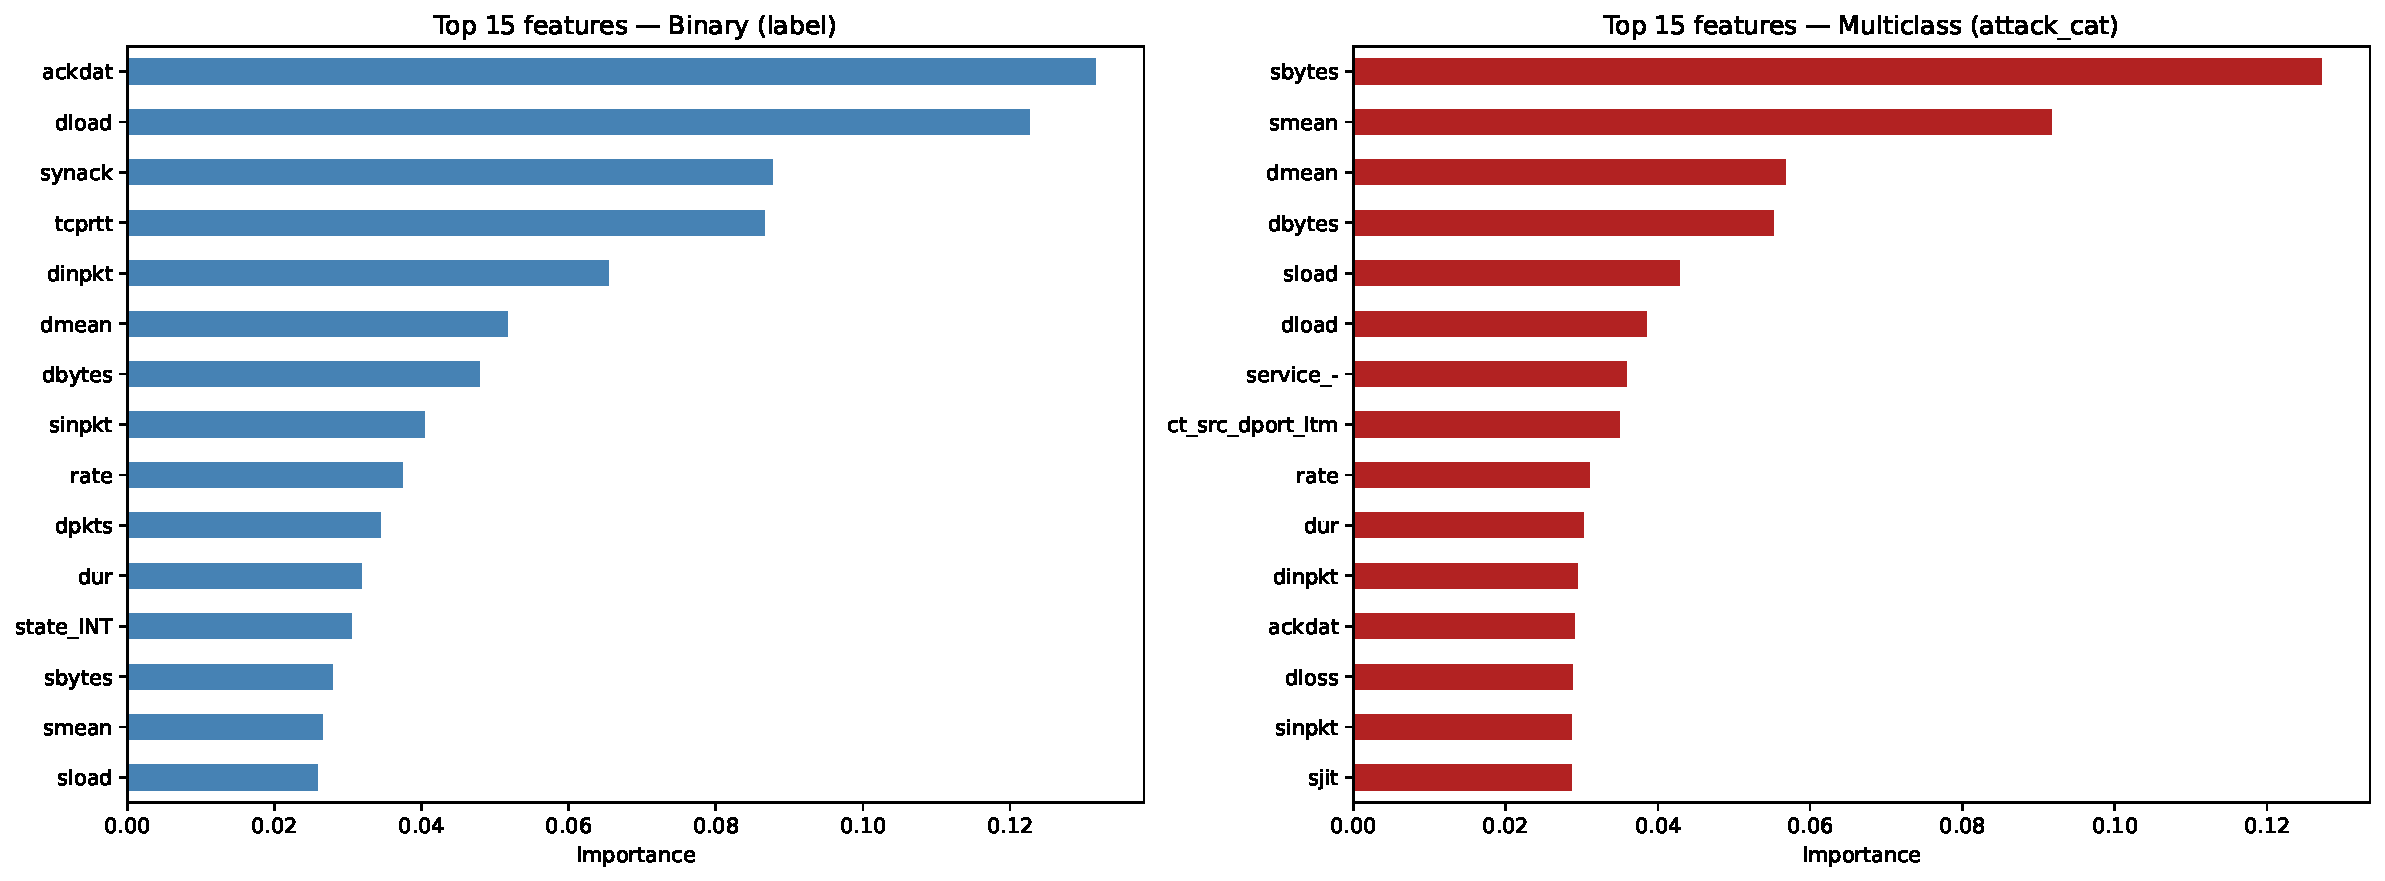
\includegraphics[width=\textwidth, height=0.55\textheight, keepaspectratio]{images/feature_importance.pdf}
\end{frame}

\section{Conclusioni}

\begin{frame}{Valutazione Progetto}
  \begin{itemize}
    \item \textbf{Trade-off metodologici}: favorire l'interpretabilità 
      (SelectKBest e modelli ad albero) si è rivelato altamente efficace per la detection binaria, ottenendo un F1-Score di 0.92 pur mantenendo regole decisionali trasparenti
    \vspace{0.2cm}
    \item \textbf{Il limite del Multiclasse}: differenziare i singoli vettori di attacco rimane intrinsecamente difficile (Macro F1: 0.57). La matrice di confusione ha rivelato una forte sovrapposizione tra categorie correlate (e.g. DoS/Exploits, Backdoor/Analysis) e, in particolare, tra Fuzzers e traffico Normal
    \vspace{0.2cm}
    \item \textbf{Dipendenza dalla Qualità dei Dati}: Il progetto ha mostrato come l'estremo sbilanciamento delle classi limiti pesantemente l'upper bound teorico delle performance di qualsiasi classificatore standard
  \end{itemize}
\end{frame}

\begin{frame}{Sviluppi Futuri}
  Per superare i limiti attuali e portare il sistema verso un Network Intrusion Detection System (NIDS) realistico, iterazioni future potrebbero esplorare:
  
  \vspace{0.3cm}
  \begin{itemize}
    \item \textbf{Resampling Avanzato}: nonostante SMOTE sia stato inizialmente valutato, è stato scartato a causa dell'estremo overhead computazionale. Lavori futuri dovranno indagare tecniche di campionamento altamente ottimizzate e scalabili
    \vspace{0.2cm}
    \item \textbf{Architetture Alternative}: Valutare classificatori non basati su alberi per determinare se confini matematici differenti possano isolare meglio classi rare
    \vspace{0.2cm}
    \item \textbf{Feature Engineering di Dominio}: derivare nuove feature di rete altamente specifiche, mirate a distinguere meglio la sovrapposizione delle firme degli attacchi minoritari rispetto alle anomalie più frequenti
  \end{itemize}
\end{frame}

\end{document}